\documentclass[preprint,prl]{revtex4}

\usepackage{ORI_Group_style}
\graphicspath{{./figs/}}

\begin{document}

\title{Photophysics of Nitrogen Vacancy centres in Nanodiamonds}
  
\author{Reece P. Roberts$^{1,2}$}
\author{Author2$^{1,2}$}

\affiliation{$^1$ Department of Physics \& Astronomy, Macquarie University, NSW 2109, Australia}
\affiliation{$^2$ ARC Centre for Engineered Quantum Systems, Macquarie University, NSW 2109, Australia}


\begin{abstract}
Lorem ipsum dolor sit amet, consectetur adipiscing elit, sed do eiusmod tempor incididunt ut labore et dolore magna aliqua. Ut enim ad minim veniam, quis nostrud exercitation ullamco laboris nisi ut aliquip ex ea commodo consequat. Duis aute irure dolor in reprehenderit in voluptate velit esse cillum dolore eu fugiat nulla pariatur. Excepteur sint occaecat cupidatat non proident, sunt in culpa qui officia deserunt mollit anim id est laborum.
\end{abstract}

\maketitle

\section{Introduction}
The Nitrogen Vacancy (NV) centre is is a point defect consisting of a nitrogen-vacancy lattice pair embedded along the [111] axis of a diamond (???ref1). The NV centre has two stable charge states, the neutral charge state (NV$^0$) and the negatively charged state (NV$^-$), with photo-induced interconversion between these two states (???ref2). The NV$^-$ charge state is an intensively studied material that has shown a wide range of applications in both Physics and Biology due to it's high stability and interesting optical properties. Biologists have used them extensively for biolabelling and imaging of internal biological structures (???ref3). For example the surface of nanodiamonds can be functionalised and internalised by cells without toxic effects and once on the target they can be imaged by using the unique optical properties of the embedded defect(???ref4). Meanwhile, Physisits have been investigating their uses in wide range of nanoscale sensing and quantum sensing(???ref5). By exploiting the quantum mechanical interactions of the defects internal spin state the NV$^-$ centre has been used to observe quantum behaviour at room temperature, providing a platform to study a wide variety of quantum manipulation protocols (???ref6). However these effects rely only on the NV$^-$ charge state and often neglect the  existence of the NV$^0$ charge state. 

The excitation photophyics of the NV centre was investigated in order to determine how to obtain the largest charge state polarisation in the NV$^-$ charge state(ref7???). Excitation wavelengths from 450-610nm were probed and an optimal excitation wavelength stated to be around 510-540nm, although the charge state polarisation was always $\leq$45\%. For most applications invoving NV centres an excitation wavelelngth in the region was chosen, typically 532nm, and the effects of the NV$^0$ charge state were ignored.

The NV has long been stated to be extremely robust, with no bleaching or blinking under normal conditions(ref8???). However, in many cases once a second probe laser is used in an experiment the Fluorescence of the NV centre is dramatically quenched(ref9???) limiting its use in further applications and in conjunction with other systems. The quenching of fluorescence has been described (???1). In contrast to these mechanisms we are collecting the fluorescence of the both charge states as well as probing in a non resonant continuous-wave regime of a few 10s of milliwats eliminating many of the above mechanisms. Interestingly the quenching mechanism at ~780nm has been observed and used and described as stimulated emission (STED) imaging(ref10???). Recently in the field is has been noted that this effect is not a true STED process, however it still gives s similar desirable effect (ref11???).  


In this paper we investigate the quenching effects of the NV centre fluorescence in order to provide insight into the charge and spin state photo-dynamics. Our process is to measure the quenching dynamics of the NV centre under steady state illumination and using established physics of the NV centre, develop a rate equation models to describe the photo-physics of the system. Using this model various assumptions are analysed to determine their validity and the most likely model that represents the photo-physics is determined by the Aikike information criteria. We believe this new rate equation model has now identified the underlying physics leading to the quenching of fluorescence of NV centres and it now allows us to predictively simulate and optimise the effect. By understanding the appropriate rates we can apply particular initialisation processes to increase the spin and charge state polarisation of the NV centre which will lead to direct enhancements of existing applications including applications such as STED like imaging and enhancing state preparation for NV based quantum technologies.

\section{Experiment}

In our experiment, (???2) type and size nanodiamonds are dispersed on a glass coverslip placed on the sample plane of a custom built scanning confocal microscope. The NV centres are pumped with a 532nm continuous wave laser after focusing through a x.xNA, Brand, type immersion objective lens ???3. The 780nm and 1042nm lasers are combined and then superimposed with the 532nm laser before the objective lens. The flourescence is collected through the same objective and sent to an avalanche photodiode. A permanent neodymium magnet was placed on a moveable arm above the sample plane so that a large non zero magnetic field could be brought in close proximity to the nanodiamond. The setup is shown in figure???. insert figure of setup.

\begin{figure}[t]
  \centering
  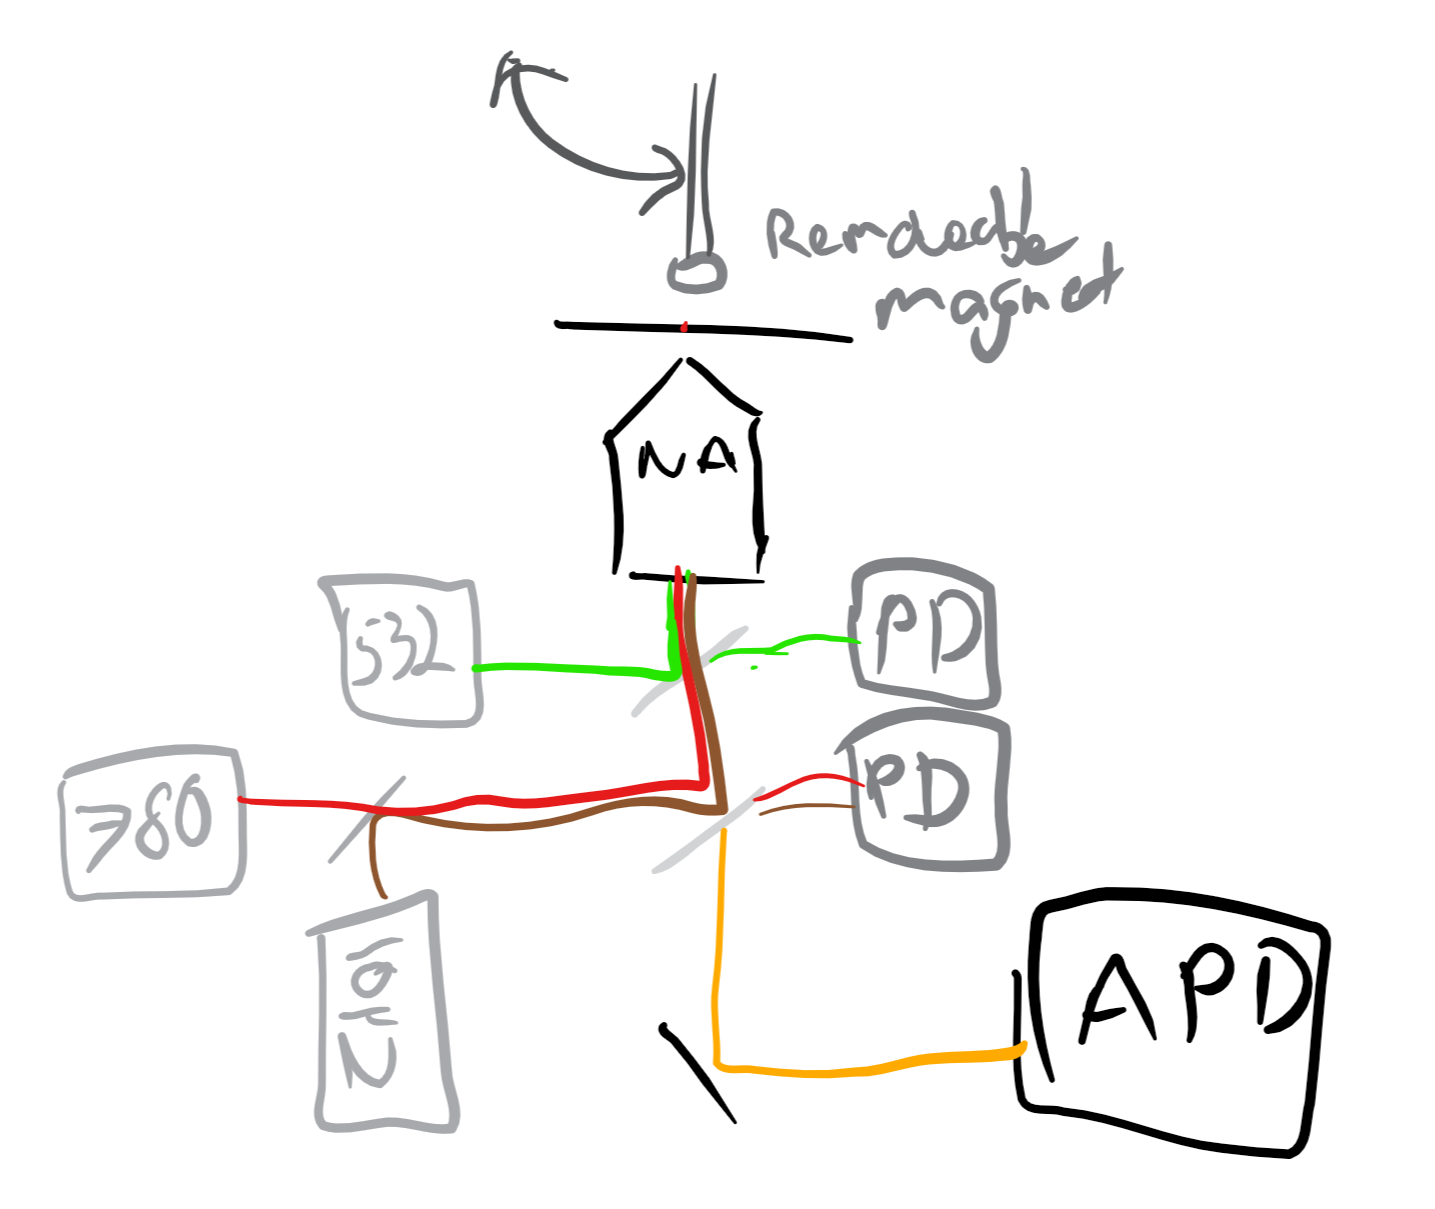
\includegraphics[width=0.5\textwidth]{Setup.png} 
 \caption{\textbf{Experimental approach.} This is the setup ???} \label{FigSetup}
\end{figure}

We start by collecting a saturation curve of the fluorescence of the NV centre. We then investigate the power dependance of the fluorescence on each of the NIR lasers for ??? powers of the green. We place a neodymium magnet ~0.5mm above the sample plane of the confocal microscope in order to mix the spin state of the NV- charge state as described in \S model. Once placed we repeated the above set of measurement. This was repeated for x??? nanodiamonds. The NIR power dependance on the fluorescence of ND??? at ???uW of 532nm plotted in Fig a. (one with most quenching) shows that ??mW of NIR laser can suppress fluorescence over ???\%.

\begin{figure}[t]
  \centering
  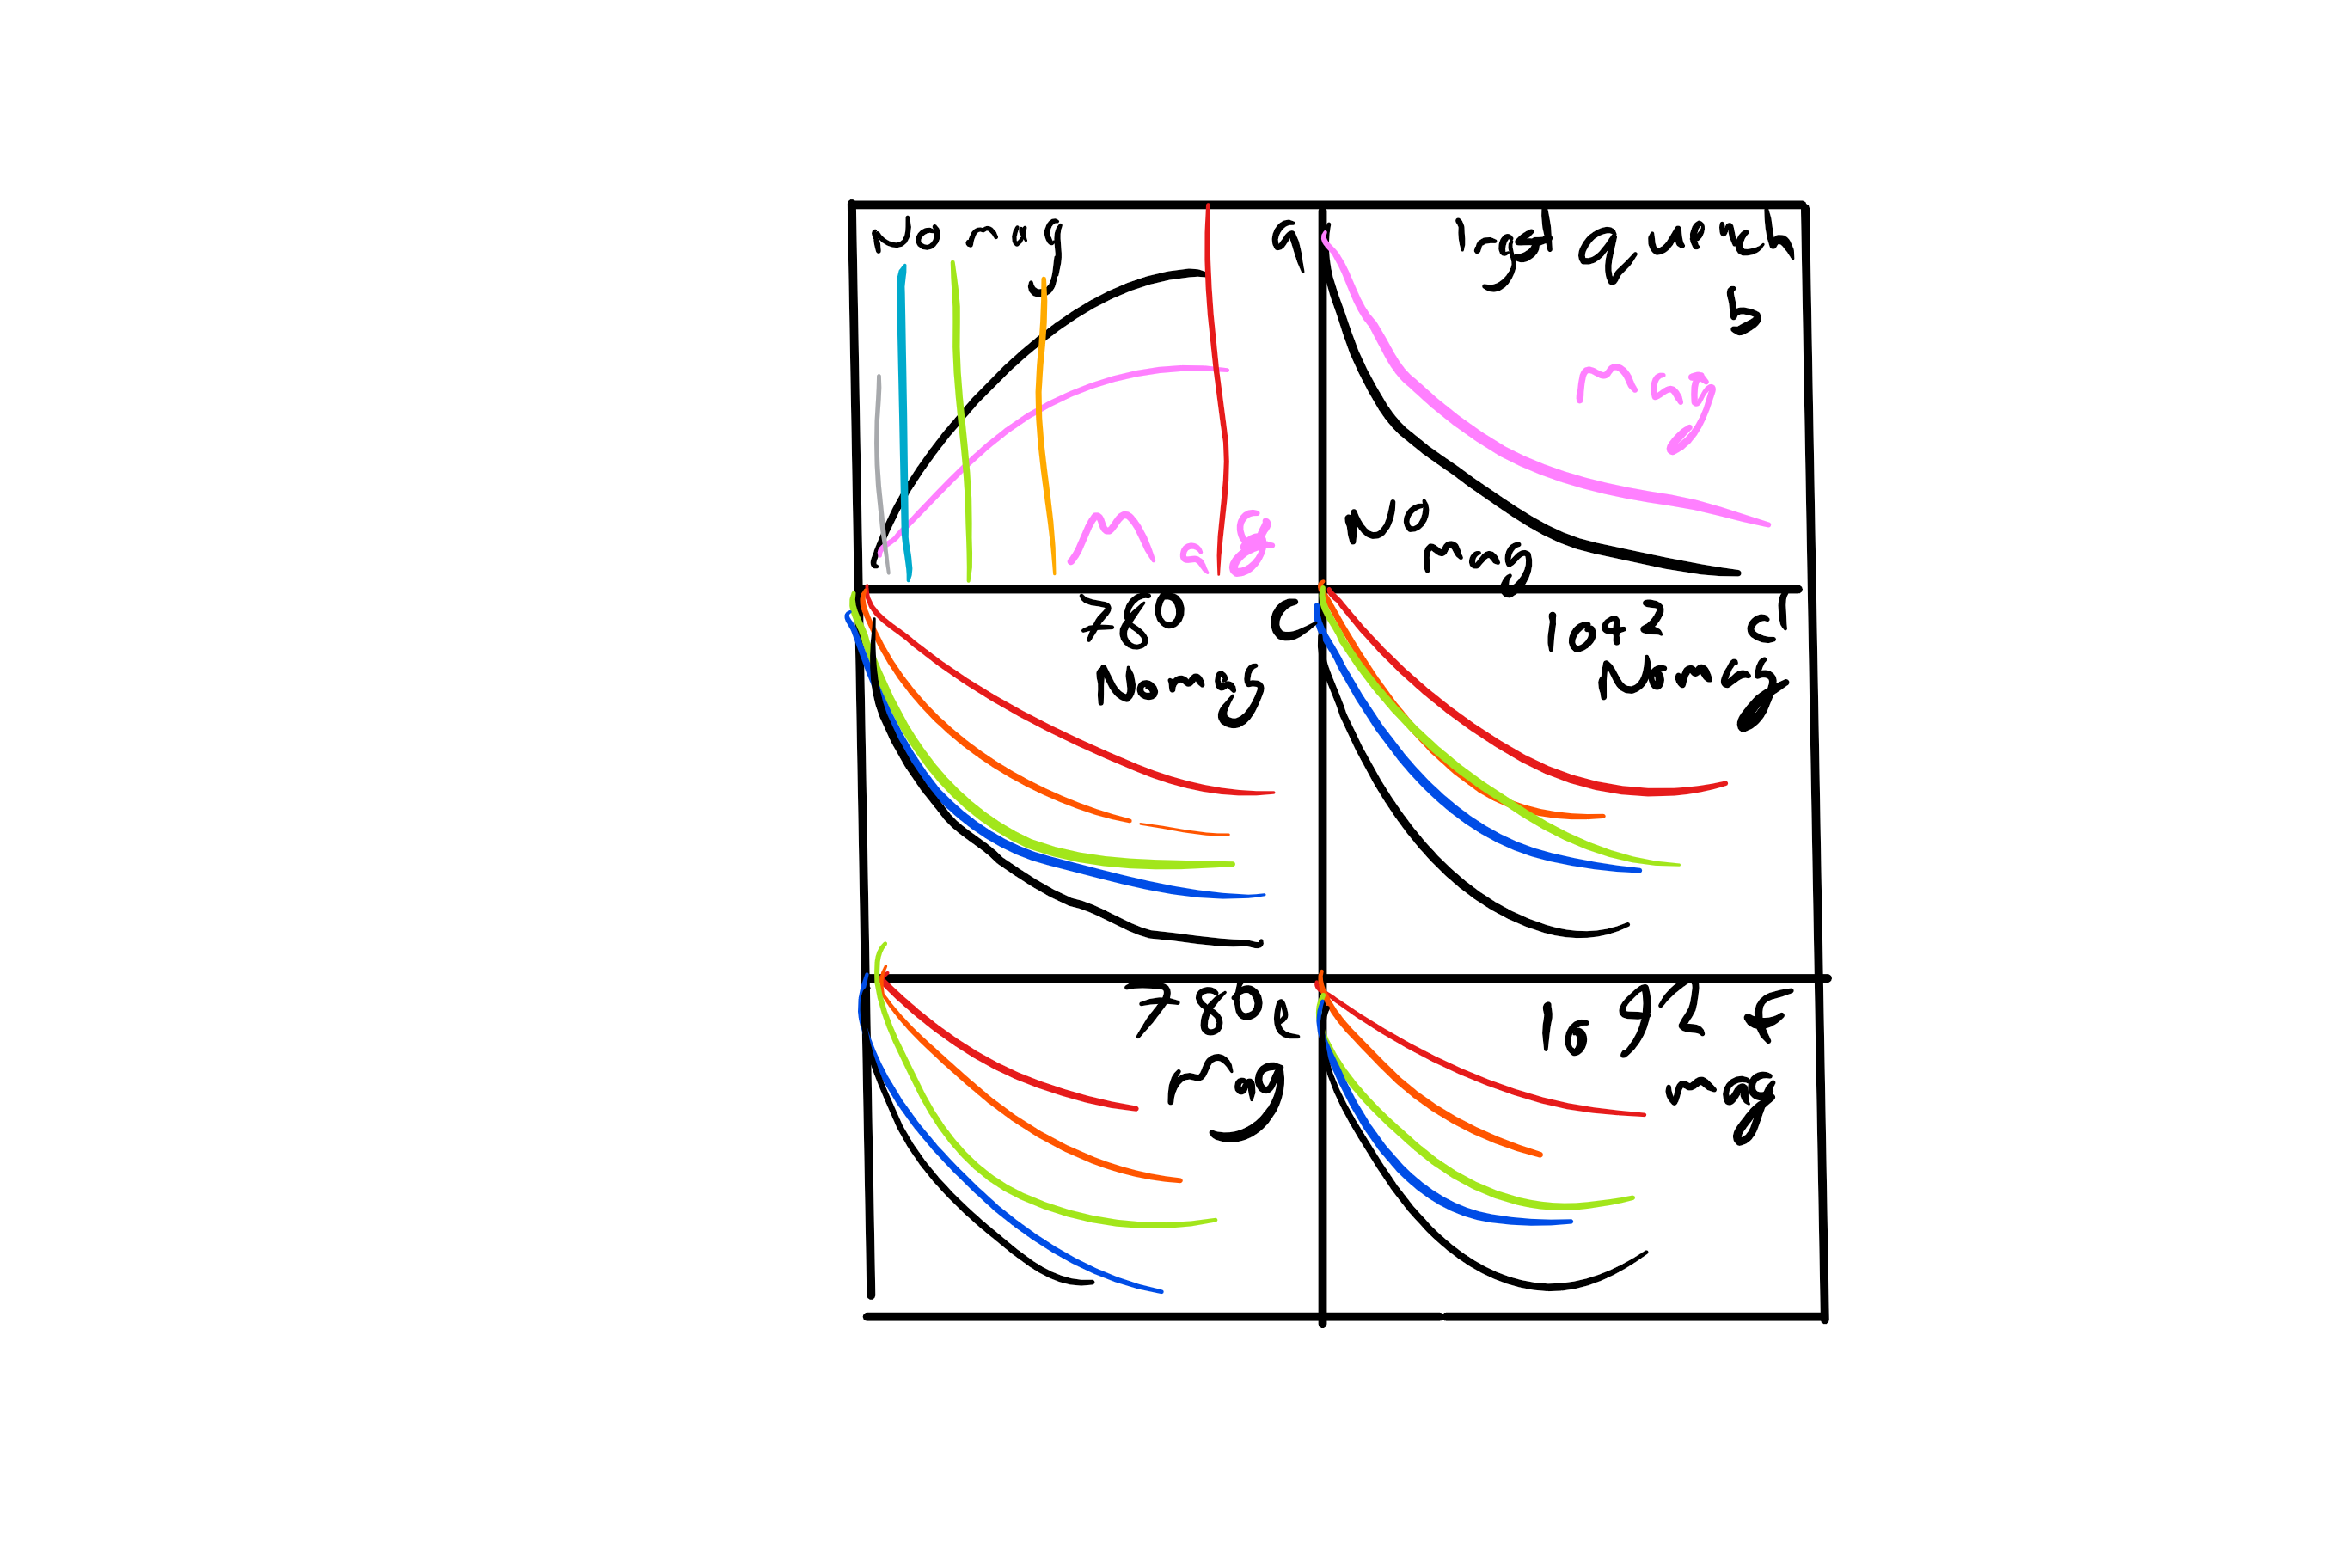
\includegraphics[width=1\textwidth]{Data.png} 
 \caption{\textbf{Experimental data.} \textbf{a.} This is the data swap a and b???} \label{FigSetup}
\end{figure}

\todo{Describe what the data is and what it indicates.}
\todo{I many also want to look at the quenching isolating each window to have an indication if the charge states are quenching equally or not}

\section{Model}



~\cite{Blancquaert2013} 

%\begin{figure}[t]
%  \centering
%  \includegraphics{figure_2D_setup.eps} 
%  \caption{\textbf{Experimental approach.} \textbf{a,} figa\textbf{b,} figb} \label{FigSetup}
%\end{figure}

%Fig.~\ref{FigAperture}.
%
%\todo{If I can find the original data, I want to treat the "old" data with the new code. In any case, I want to redo the plot with the same colorscale as Fig2.}


\section*{Acknowledgements}

....
%%%%%%%%%%%%%%%%%%%%%%%%%%%%%%%%%%%%%%%%%
%%%%%%%%%%%%%%%%%%%%%%%%%%%%%%%%%%%%%%%%%
%%%%%                                                                                                   %%%%%
%%%%%                                       APPENDIX                                          %%%%%
%%%%%                                                                                                   %%%%%
%%%%%%%%%%%%%%%%%%%%%%%%%%%%%%%%%%%%%%%%%
%%%%%%%%%%%%%%%%%%%%%%%%%%%%%%%%%%%%%%%%%

%
%\appendix
%
%\section{Experimental parameters}
%\label{param}
%




\begin{thebibliography}{27}






\end{thebibliography}




\end{document}
